%
%===============>>  ГРУППА 10-2 МОДУЛЬ 4  <<=============
%
\setmodule{4}
%
%===============>>  Занятие 1  <<===============
%
\begin{class}[number=1]
	\begin{listofex}
		%		В ДЗ №1
		%		\item Вычислить рациональным способом:
		%		\begin{enumcols}[itemcolumns=3]
		%			\item \( \sqrt{16+4\cdot4\cdot24} \)
		%			\item \( \sqrt{83^3\cdot2^2-83^2\cdot2^3} \)
		%			\item \( \sqrt{50^2-4\cdot7\cdot7} \)
		%		\end{enumcols}
		\item Построить график функции \( y=2x-5 \).
		\begin{enumcols}[itemcolumns=1]
			\item Принадлежит ли точка с координатами \( (112;217) \) графику этой функции?
			\item Найти точку пересечения графика данной функции с графиком функции \( y=4x-1 \).
		\end{enumcols}
		\item Построить графики функций \( f(x)=x^2-2x+1 \) и \( g(x)=x^2+6x+8 \).\\
		Выберите верные утверждения:
		\begin{enumcols}[itemcolumns=4]
			\item \( f(-1)>f(1) \);
			\item \( g(-1)<f(-1) \);
			\item \( g(-2)=f(1) \);
			\item \( f(3)<g(-5) \);
		\end{enumcols}
		\begin{enumcols}[itemcolumns=1, resume]
			\item график функции \( f(x) \) возрастает на промежутке \( [0;+\infty) \);
			\item график функции \( g(x) \) убывает на промежутке \( [-9;-4] \);
			\item промежуток возрастания функции \( f(x) \) входит в промежуток возрастания функции \( g(x) \);
			\item \( f(x)=4 \) при \( x=3 \);
			\item наименьшее значение функция \( f(x) \) принимает в \( x=-1 \);
			\item наименьшее значение \( f(x) \) меньше наименьшего значения \( g(x) \);
			\item корнем уравнения \( f(x)=9 \) является только \( x=-2 \);
			\item \( f(x)\ge0 \) при любом \( x \);
			\item \( g(x)\le0 \) при \( x\in[-4;-2] \);
			\item график функции \( g(x) \) пересекается c осью \( Y \) в точке \( (0;4) \).
		\end{enumcols}
		\item Решить систему неравенств:
		\begin{enumcols}[itemcolumns=2]
			\item
			\( \left\{
			\begin{array}{l}
				3(x-1)-2(2-3x)>5x-3,\\
				8x-3(2x+5)<2(x-7).
			\end{array}
			\right. \)
			\item
			\( \left\{
			\begin{array}{l}
				12x-3(x-5)>2x+1,\\
				(x-7)(x+12)\le0.
			\end{array}
			\right. \)
		\end{enumcols}
		\item При каких значениях переменной выражение \( \sqrt{4x+1}+\sqrt{2-3x} \) имеет смысл?
		\item Построить график функции \( f(x)=\sqrt{x-4}+1 \).
		\begin{enumcols}[itemcolumns=1]
			\item определить область определения и область значений функции;
			\item сравнить \( f(7) \) и \( f(12) \);
			\item вычислить \( f(x)=26 \)
			\item существует ли \( x \), при котором \( f(x)=-1 \)? Объясните это графически и аналитически.
		\end{enumcols}
		\item Построить график функции \( y=x-|2x+1|-2 \).
		\begin{enumcols}[itemcolumns=1]
			\item найти точку минимума и наименьшее значение данной функции;
			\item определить промежутки возрастания и убывания функции;
			\item найти точки пересечения данного графика с графиком функции \( y=x-5 \).
		\end{enumcols}
		\item Баржа прошла по течению реки 48 км и, повернув обратно, прошла ещё 36 км, затратив на весь путь 6 часов. Найдите собственную скорость баржи, если скорость течения реки равна 5 км/ч.
	\end{listofex}
\end{class}
%
%===============>>  Занятие 2  <<===============
%
\begin{class}[number=2]
	\begin{listofex}
%		В ДЗ
%		\item Постройте графики функции \( y=4x-1 \) и \( y=-\dfrac{1}{2}x+2,5 \). Графически определите точку пересечения этих графиков. Во сколько раз ордината точки пересечения больше абсциссы?
		\item Найдите точку пересечения графиков функций \( y=12x-70 \) и \( y=6x+2 \).
		\item Постройте график функции \( f(x)=x^2-6x+8 \). Выберите верные утверждения:
		\begin{enumcols}[itemcolumns=1]
			\item График функции возрастает на промежутке \( [4;+\infty) \);
			\item График функции убывает на промежутке \( [-7;7] \);
			\item \( f(-4)<f(4) \);
			\item \( f(-1)=f(3) \);
			\item \( f(x)\ge0 \) при \( x\ge4 \);
			\item \( f(x)\ge0 \) только при \( x\ge4 \);
			\item Данный график функции пересекается с графиком \( y=-x-8 \) в двух точках.
		\end{enumcols}
		\item Подставьте вместо знака \( * \) число так, чтобы функция \( y=2x^2-3x+* \) проходила через точку с координатами \( (4;15) \). Найдите координаты вершины этой параболы. Вычислите расстояние от вершины до точки \( (4;15) \).
		
%		В ДЗ
%		\item Решить систему неравенств:
%		\[ \left\{
%		\begin{array}{l}
%			6(x+2)-4(0,5-2x)>2x-6,\\
%			9x+x(2x+5)<2(x^2-7).
%		\end{array}
%		\right. \]

%		В ДЗ
%		\item \exercise{177}
%		\item \exercise{189}

		\item При каких значениях переменной выражение \( \sqrt{12x-6}+\sqrt{4-5x} \) имеет смысл?
		\item \exercise{1240}
		\item \exercise{24}
		\item \exercise{1855}
		\item Высота равностороннего треугольника равна \( 15\sqrt{3} \). Найдите его периметр.
	\end{listofex}
\end{class}
%
%===============>>  Домашняя работа 1  <<===============
%
\begin{homework}[number=1]
	\begin{listofex}
		\item Вычислить рациональным способом:
		\begin{enumcols}[itemcolumns=3]
			\item \( \sqrt{16+4\cdot4\cdot24} \)
			\item \( \sqrt{83^3\cdot2^2-83^2\cdot2^3} \)
			\item \( \sqrt{50^2-4\cdot7\cdot7} \)
		\end{enumcols}
		\item Постройте графики функции \( y=4x-1 \) и \( y=-\dfrac{1}{2}x+2,5 \). Графически определите точку пересечения этих графиков. Во сколько раз ордината точки пересечения больше абсциссы?
		\item Решить систему неравенств:
		\[ \left\{
		\begin{array}{l}
			6(x+2)-4(0,5-2x)>2x-6,\\
			9x+x(2x+5)<2(x^2-7).
		\end{array}
		\right. \]
		\item \exercise{177}
		\item \exercise{189}
		\item Построить график функции \( f(x)=\sqrt{10-x}+5 \).
		\begin{enumcols}[itemcolumns=1]
			\item определить область определения и область значений функции;
			\item сравнить \( f(-6) \) и \( f(6) \);
			\item вычислить \( f(x)=17 \)
			\item существует ли \( x \), при котором \( f(x)=15 \)? Объясните это графически и аналитически.
		\end{enumcols}
		\item Постройте график функции \( f(x)=x^2+6x+5 \). Выберите верные утверждения:
		\begin{enumcols}[itemcolumns=1]
			\item График функции возрастает на промежутке \( [-5;+\infty) \);
			\item График функции убывает на промежутке \( [-7;-2,5] \);
			\item \( f(-5)<f(-1) \);
			\item \( f(0)=f(-6) \);
			\item \( f(x)\ge0 \) при \( x\ge1 \);
			\item \( f(x)\ge0 \) только при \( x\ge1 \);
			\item Данный график функции пересекается с графиком \( y=x-1 \) в двух точках.
		\end{enumcols}
	\end{listofex}
\end{homework}
%
%===============>>  Занятие 3  <<===============
%
\begin{class}[number=3]
	\begin{listofex}
		\item Вычислить:
		\begin{enumcols}[itemcolumns=4]
			\item \( \dfrac{\left( 5^{3/5}\cdot7^{2/3} \right)^{15}}{39^9} \)
			\item \( 20^{-3,9}\cdot5^{2,9}:4^{-4,9} \)
			\item \( \dfrac{32^{-9}\cdot8^4}{\left( 4^{-8} \right)^2} \)
			\item \( \dfrac{\sqrt[3]{81}\cdot\sqrt[4]{81}}{\sqrt[12]{81}} \)
		\end{enumcols}
		\item \exercise{1867}
		\item 
		\begin{minipage}[t]{0.67\textwidth}
			На рисунке изображены графики функций \( f(x)=\dfrac{k}{x} \) и \( g(x)=ax+b \), которые пересекаются в точках \( A \) и \( B \). Найдите абсциссу точки \( B \).
		\end{minipage}
		\begin{minipage}[c]{0.25\textwidth}
			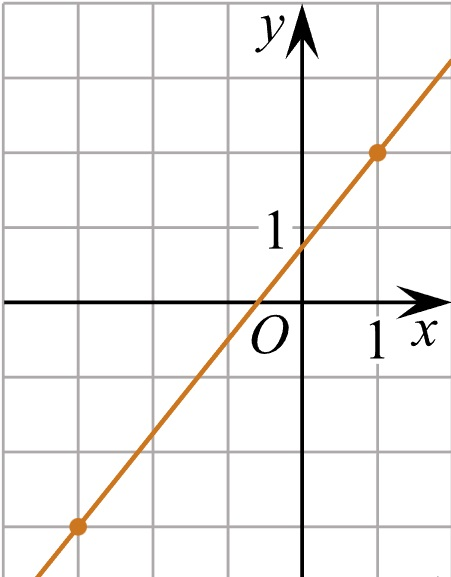
\includegraphics[align=t, width=\textwidth]{./pics/G101M4C4-1}
		\end{minipage}
		\item 
		\begin{minipage}[t]{0.67\textwidth}
			На рисунке изображены графики функций \( f(x)=k\sqrt{x} \). Найдите \( f(6,76) \).
		\end{minipage}
		\begin{minipage}[c]{0.25\textwidth}
			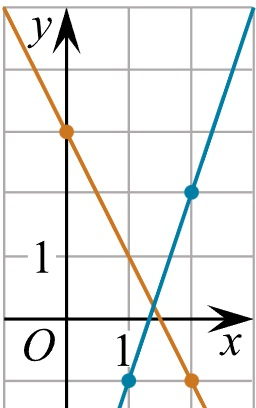
\includegraphics[align=t, width=\textwidth]{./pics/G101M4C4-2}
		\end{minipage}
		\item Решите уравнение: \( (x^2-25)\cdot\sqrt{8+2x-x^2}=(25-x^2)\cdot\sqrt{x+2} \)
		\item Расстояние между пристанями \( A \) и \( B \) равно \( 63 \) км. Из \( A \) в \( B \) по течению реки отправился плот, а через \( 1 \) час вслед за ним отправилась яхта, которая прибыла в пункт \( B \), а через \( 1 \) час отправилась обратно и возвратилась в A. К этому времени плот проплыл \( 20 \) км. Найдите скорость яхты в неподвижной воде, если скорость течения реки равна \( 2 \) км/ч. Ответ дайте в км/ч.
		\item Дан куб, сумма площадей граней которого равна \( 24 \), и дан прямоугольный
		параллелепипед \( ABCDA_1B_1C_1D_1 \). Ребро \( AB \) прямоугольного
		параллелепипеда меньше ребра куба на \( 1 \), ребро \( AD \) --- больше ребра куба
		на \( 1 \), а ребро \( AA_1 \) --- равно ребру куба. Найдите сумму площадей граней
		прямоугольного параллелепипеда \( ABCDA_1B_1C_1D_1 \).
		\item Около трапеции описана окружность. Периметр трапеции равен \( 36 \),
		средняя линия равна \( 8 \). Найдите длину боковой стороны трапеции.
	\end{listofex}
\end{class}
%
%===============>>  Занятие 4  <<===============
% смещение на одно занятие с прошлого месяца
%\begin{class}[number=4]
%	\begin{listofex}
%		\item Пусто
%	\end{listofex}
%\end{class}
%
%===============>>  Домашняя работа 2  <<===============
%
%\begin{homework}[number=2]
%	\begin{listofex}
%
%	\end{listofex}
%\end{homework}
%
%===============>>  Занятие 5  <<===============
% смещение на одно занятие с прошлого месяца
%\begin{class}[number=5]
%	\begin{listofex}
%		\item Пусто
%	\end{listofex}
%\end{class}
%
%===============>>  Домашняя работа 3  <<===============
%
%\begin{homework}[number=2]
%	\begin{listofex}
%
%	\end{listofex}
%\end{homework}
%\newpage
%\title{Подготовка к проверочной работе}
%\begin{listofex}
%	
%\end{listofex}
%
%===============>>  Занятие 7  <<===============
%
%\begin{class}[number=7]
%	\begin{listofex}
%	
%	\end{listofex}
%\end{class}
%
%===============>>  Провечная работа  <<===============
%
%\begin{exam}
%	\begin{listofex}
%	
%	\end{listofex}
%\end{exam}